\documentclass[aspectratio=1610, 13pt]{beamer}
\usepackage{xcolor}
\usepackage{multicol}
\usepackage{mathtools,array}
\usepackage[T1]{fontenc}
\usepackage{autobreak}
\usepackage{algorithm}
\usepackage{algorithmic}
\usepackage{listings}
\usepackage{stmaryrd}
\usepackage{dutchcal}
\usepackage{zi4}
\usepackage[font={scriptsize,bf}]{caption}
% \usepackage{subcaption}
\usepackage{graphics}
\usepackage{tikz}
\usepackage{fontawesome5}
\usepackage{mathpartir}

\newcommand{\naturals}{\mathbb{N}}
\newcommand{\reals}{\mathbb{R}}

\newcommand{\Dist}[1]{\mathcal{D}(#1)}
\newcommand{\expectation}{\mathbb{E}}

\newcommand{\states}{S}
\newcommand{\actions}{A}
\newcommand{\observables}{O}
\newcommand{\trans}{T}
\newcommand{\obs}{Z}
\newcommand{\reward}{R}
\newcommand{\discount}{\gamma}

\newcommand{\beliefs}{\mathcal{B}}
\newcommand{\beliefUpdate}{\tau}

\newcommand{\policy}{\pi}

\newcommand{\diff}[1]{\mathop{}\!\mathrm{d}#1}
\renewcommand{\figurename}{Figure}
\renewcommand{\refname}{Reference}

\AtBeginDocument{
  \catcode`_=12
  \begingroup\lccode`~=`_
  \lowercase{\endgroup\let~}\sb
  \mathcode`_="8000
}

% \usetheme{Madrid}
% % \usetheme{default}
% \setbeamertemplate{caption}[numbered]
% \setbeamerfont{title}{size=\large}
\mode<presentation>
{
  \usetheme{Darmstadt}      % or try Darmstadt, Madrid, Warsaw, ...
  \usecolortheme{default} % or try albatross, beaver, crane, ...
  \usefonttheme[onlymath]{serif}  % or try serif, structurebold, ...
  \setbeamertemplate{navigation symbols}{}
  \setbeamertemplate{caption}[numbered]
  \setbeamertemplate{footline}[frame number] 
} 

\usepackage{listings}
\lstdefinestyle{heaplang}{
    language=Caml,
    basicstyle=\footnotesize\ttfamily,
    keywordstyle=\color{blue},
    commentstyle=\color{red},
    escapeinside={<@}{@>},
    morekeywords={new_chan, fork, recv, send, swap, ref}
}
\lstdefinestyle{clang}{
    language=Caml,
    basicstyle=\footnotesize\ttfamily,
    keywordstyle=\color{blue},
    commentstyle=\color{red},
    escapeinside={<@}{@>},
}
\lstset{style=heaplang}

\usepackage{natbib}

\newcommand{\buchi}{B\"uchi }

\definecolor{goldenpoppy}{rgb}{0.99, 0.76, 0.0}
\definecolor{goldenyellow}{rgb}{1.0, 0.87, 0.0}
\definecolor{green2}{rgb}{0.1,0.7,0.3} 
\newcommand{\gcheck}{{\color{green2}\faCheckCircle[regular] }}
\newcommand{\rcross}{{\color{red} \faTimesCircle[regular]} }
\newcommand{\rflag}{{\color{red} \faFlag}}
% \usepackage{algorithm,amsmath}
% \usepackage[noend]{algpseudocode}

\newcommand{\zlstinline}{\let\par\endgraf\lstinline}
\newcommand{\comments}[1]{{\color{red}#1}}
\title{SAT-Based Model Checking Without Unrolling}
\author{Author: Aaron R. Bradley\\
Reporter:  Xie Li}
\date{\today}
\begin{document}
\maketitle

\begin{frame}{Compute Largest Inductive Subclause}
\[\psi \wedge c \wedge T \rightarrow c'\]
\vspace{5em}
\end{frame}

\begin{frame}{IC3: The Main Function}
The main function:
\begin{algorithmic}[1]
\STATE bool \texttt{prove}():
	\IF{sat($I \wedge \neg P \vee I \wedge T \wedge \neg P'$)}
	\RETURN \textbf{false}
	\ENDIF
	\STATE $F_0 := I$, \texttt{clauses}$(F_0) := \emptyset$
	\STATE $F_i := P$, \texttt{clauses}$(F_i) := \emptyset$ for all $i > 0$.
	\FOR{$k := 1$ to $\cdots$}
	\IF{\textbf{not} \texttt{strengthen}$(k)$}
	\RETURN  \textbf{false}
	\ENDIF
	\STATE \texttt{propagateClauses}$(k)$
	\IF{\texttt{clauses}$(F_i)$ = \texttt{clauses}$(F_{i+1} )$ for some $1 \le i \le k$}
	\RETURN \textbf{true}
	\ENDIF
	\ENDFOR
\end{algorithmic}
\end{frame}

\begin{frame}{IC3: Strengthen Function}

\begin{algorithmic}[1]
\STATE bool \texttt{strengthen}($k$ : level):
\STATE \textbf{try:}
	\WHILE{sat($F_k \wedge T \wedge \neg P'$)}
		\STATE $s:=$ the predecessor extracted from witness
		\STATE $n := $ \texttt{inductiveGeneralize}$ (s, k-2, k)$ // why $k - 2$?
		\STATE \texttt{pushGeneralization}($\{(n + 1, s)\}, k$)
	\ENDWHILE
		\RETURN \textbf{true}
\STATE \textbf{except} Counterexample:\textbf{ return false}
\end{algorithmic}
\end{frame}

\begin{frame}{IC3: Inductive Generalization Function}

\begin{algorithmic}[1]
\STATE level \texttt{inductiveGeneralize}($s$ : state, $min$: level, $k$ : level):
\IF {$min < 0$ \textbf{and} sat($F_0 \wedge T \wedge \neg s \wedge s'$)}
\STATE \textbf{raise} Counterexample
\ENDIF
\FOR{$i := \max (1, min + 1)$ to $k$}
\IF{sat($F_i\wedge T \wedge \neg s \wedge s'$)}
\STATE \texttt{generateClause}$(s, i-1, k)$
\RETURN $i - 1$
\ENDIF
\ENDFOR
\STATE \texttt{generateClause}$(s, i-1, k)$
\RETURN $k$
\end{algorithmic}
\begin{algorithmic}[1]
\STATE void \texttt{generateClause}$(s, i, k)$: find inductive subclause of $\neg s$ for $F_0, F_1, \ldots, F_{i + 1}$ and conjoin it to them respectively.
\end{algorithmic}
\end{frame}

\begin{frame}{IC3: pushGeneralization Function}
\begin{algorithmic}[1]
\STATE void \texttt{pushGeneralization}($states$ : (level ,state) set,  $k$ : level):
\WHILE{\textbf{true}}
	\STATE $(n, s) := $ choose from $states$, minimizing $n$.
	\IF{$n > k$}
		\RETURN
	\ENDIF
	\IF{sat($F_n \wedge T \wedge s'$)}
		\STATE $p := $ the predecessor extracted from the witness
		\STATE $m := $\texttt{inductivelyGeneralize}($p, n-2, k$)// same reason for $n-2$
		\STATE $states := states \cup \{(m + 1, p)\}$
	\ELSE
		\STATE $m := $\texttt{inductivelyGeneralize}($s, n, k$)
		\STATE $states := states\backslash\{n, s\} \cup \{(m + 1, s)\}$
	\ENDIF

\ENDWHILE
\end{algorithmic}
\end{frame}

\begin{frame}{A Demo Example}

\end{frame}
\begin{frame}{A Demo Example}

\end{frame}

\begin{frame}{Total Correctness}
\begin{theorem}
For finite transition system $S$ and safety property $P$ the algorithm terminates and it returns true if and only if $P$ is $S$-invariant.
\end{theorem}
\end{frame}


\begin{frame}{Parallel Implementation}
	Finding inductive subclauses can be done in parallel and communicate through central server.
	
Experimental result:
\begin{center}
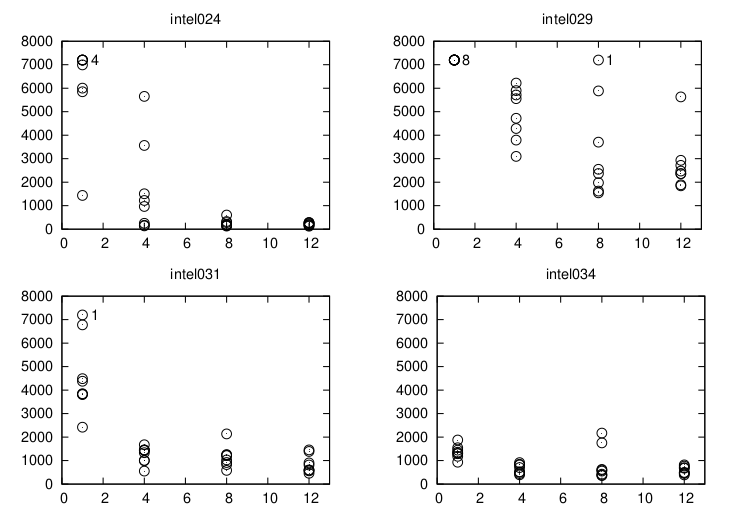
\includegraphics[scale=0.28]{para.png}
\end{center}
\end{frame}

\begin{frame}{Further Questions}
\begin{itemize}
\item What about infinite transition system?
\item What about more general transition system?
\end{itemize}
\end{frame}
\end{document}